\chapter{Creating an Efficient Database Infrastructure for Discovery of Real Materials Exemplified with High Entropy Alloys} \label{chap:ultera}

\section{Introduction} \label{ultera:sec:intro}
\todo

\cite{Debnath2021GenerativeAlloys}
\cite{Debnath2023ComparingAlloys}
\cite{Li2024DesignExperiments}

\begin{figure}[H]
    \centering
    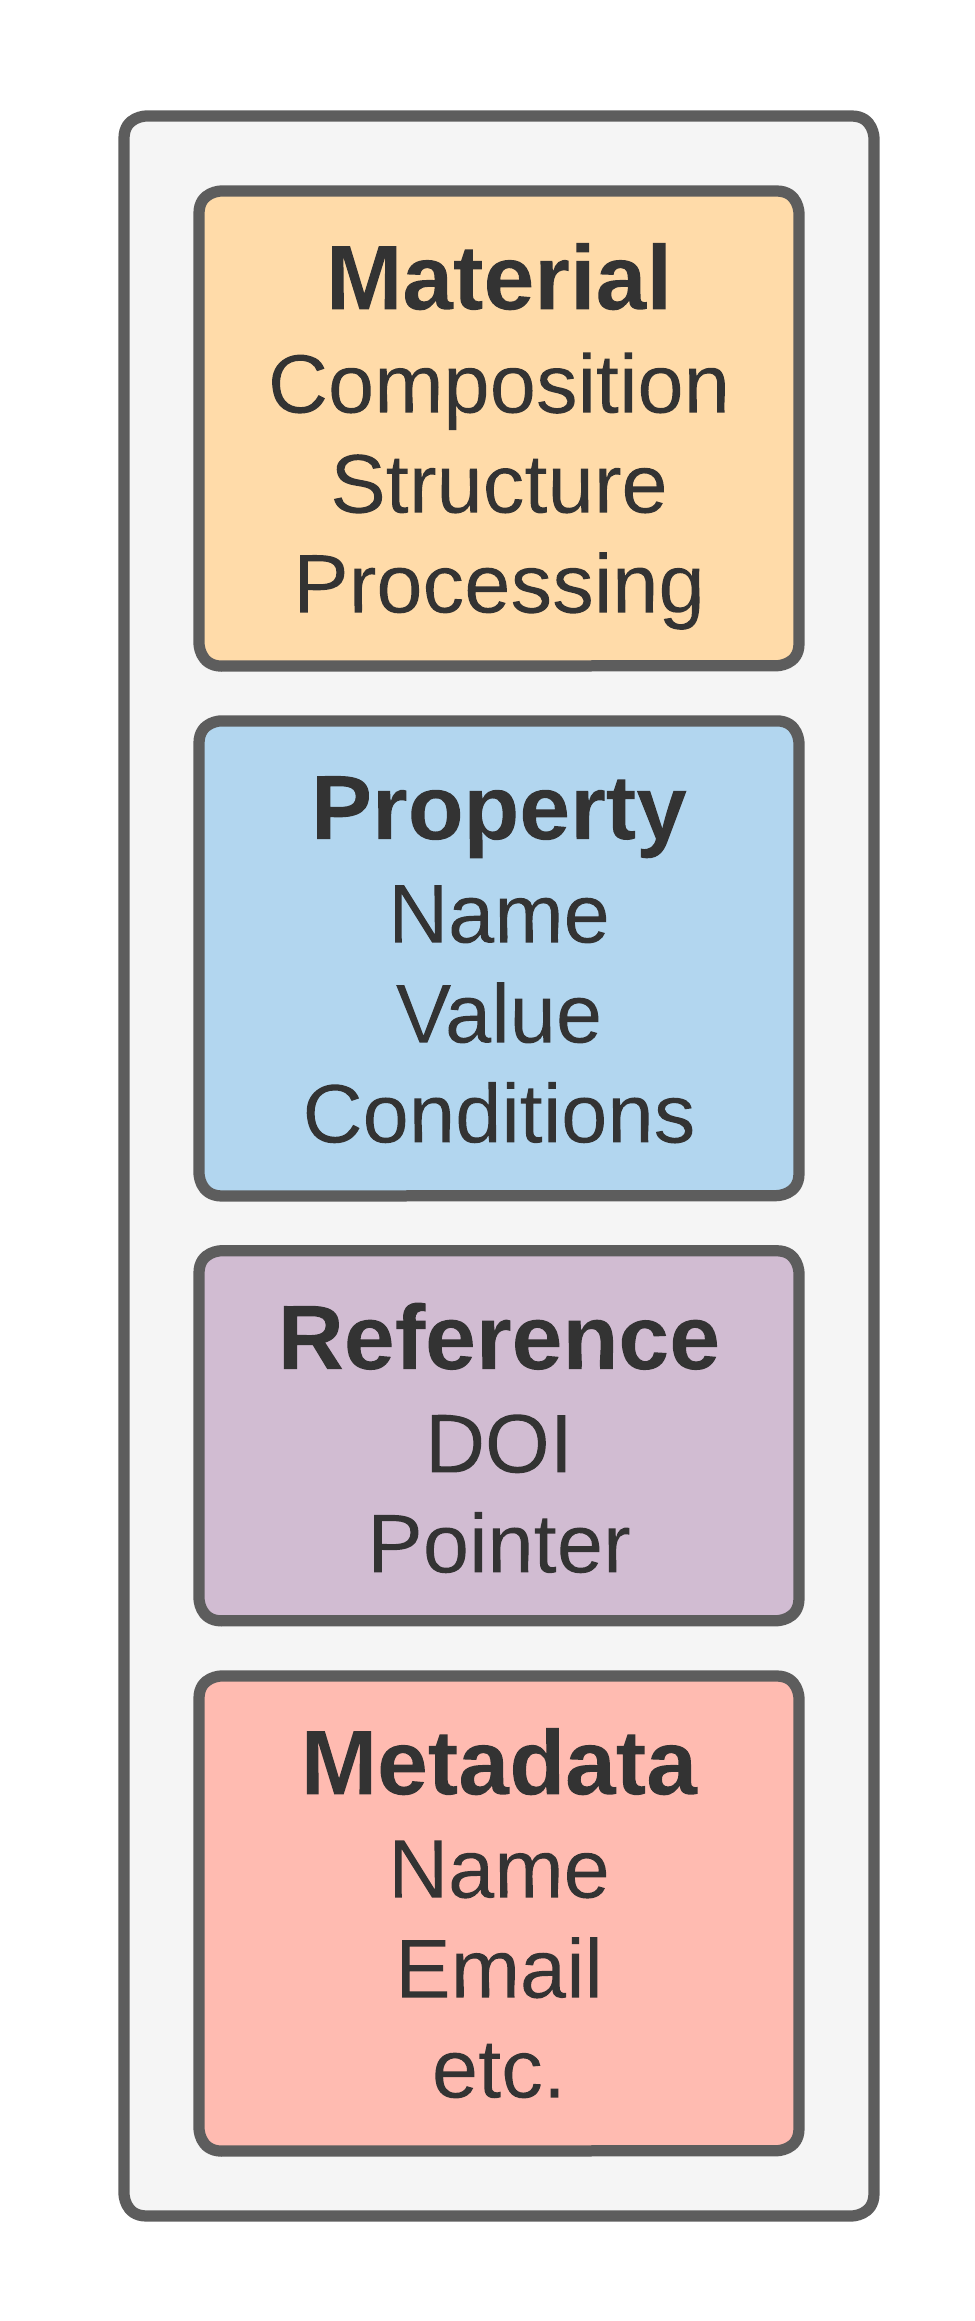
\includegraphics[width=0.2\textwidth]{ultera/ULTERA Data Detail_material.png}
    \caption{Underlying core data overview.}
    \label{ultera:fig:material}
\end{figure}


\section{Dataset} \label{ultera:sec:datadescription}
\newcommand{\statisticstime}{April 2024}

\todo

\begin{figure}[H]
    \centering
    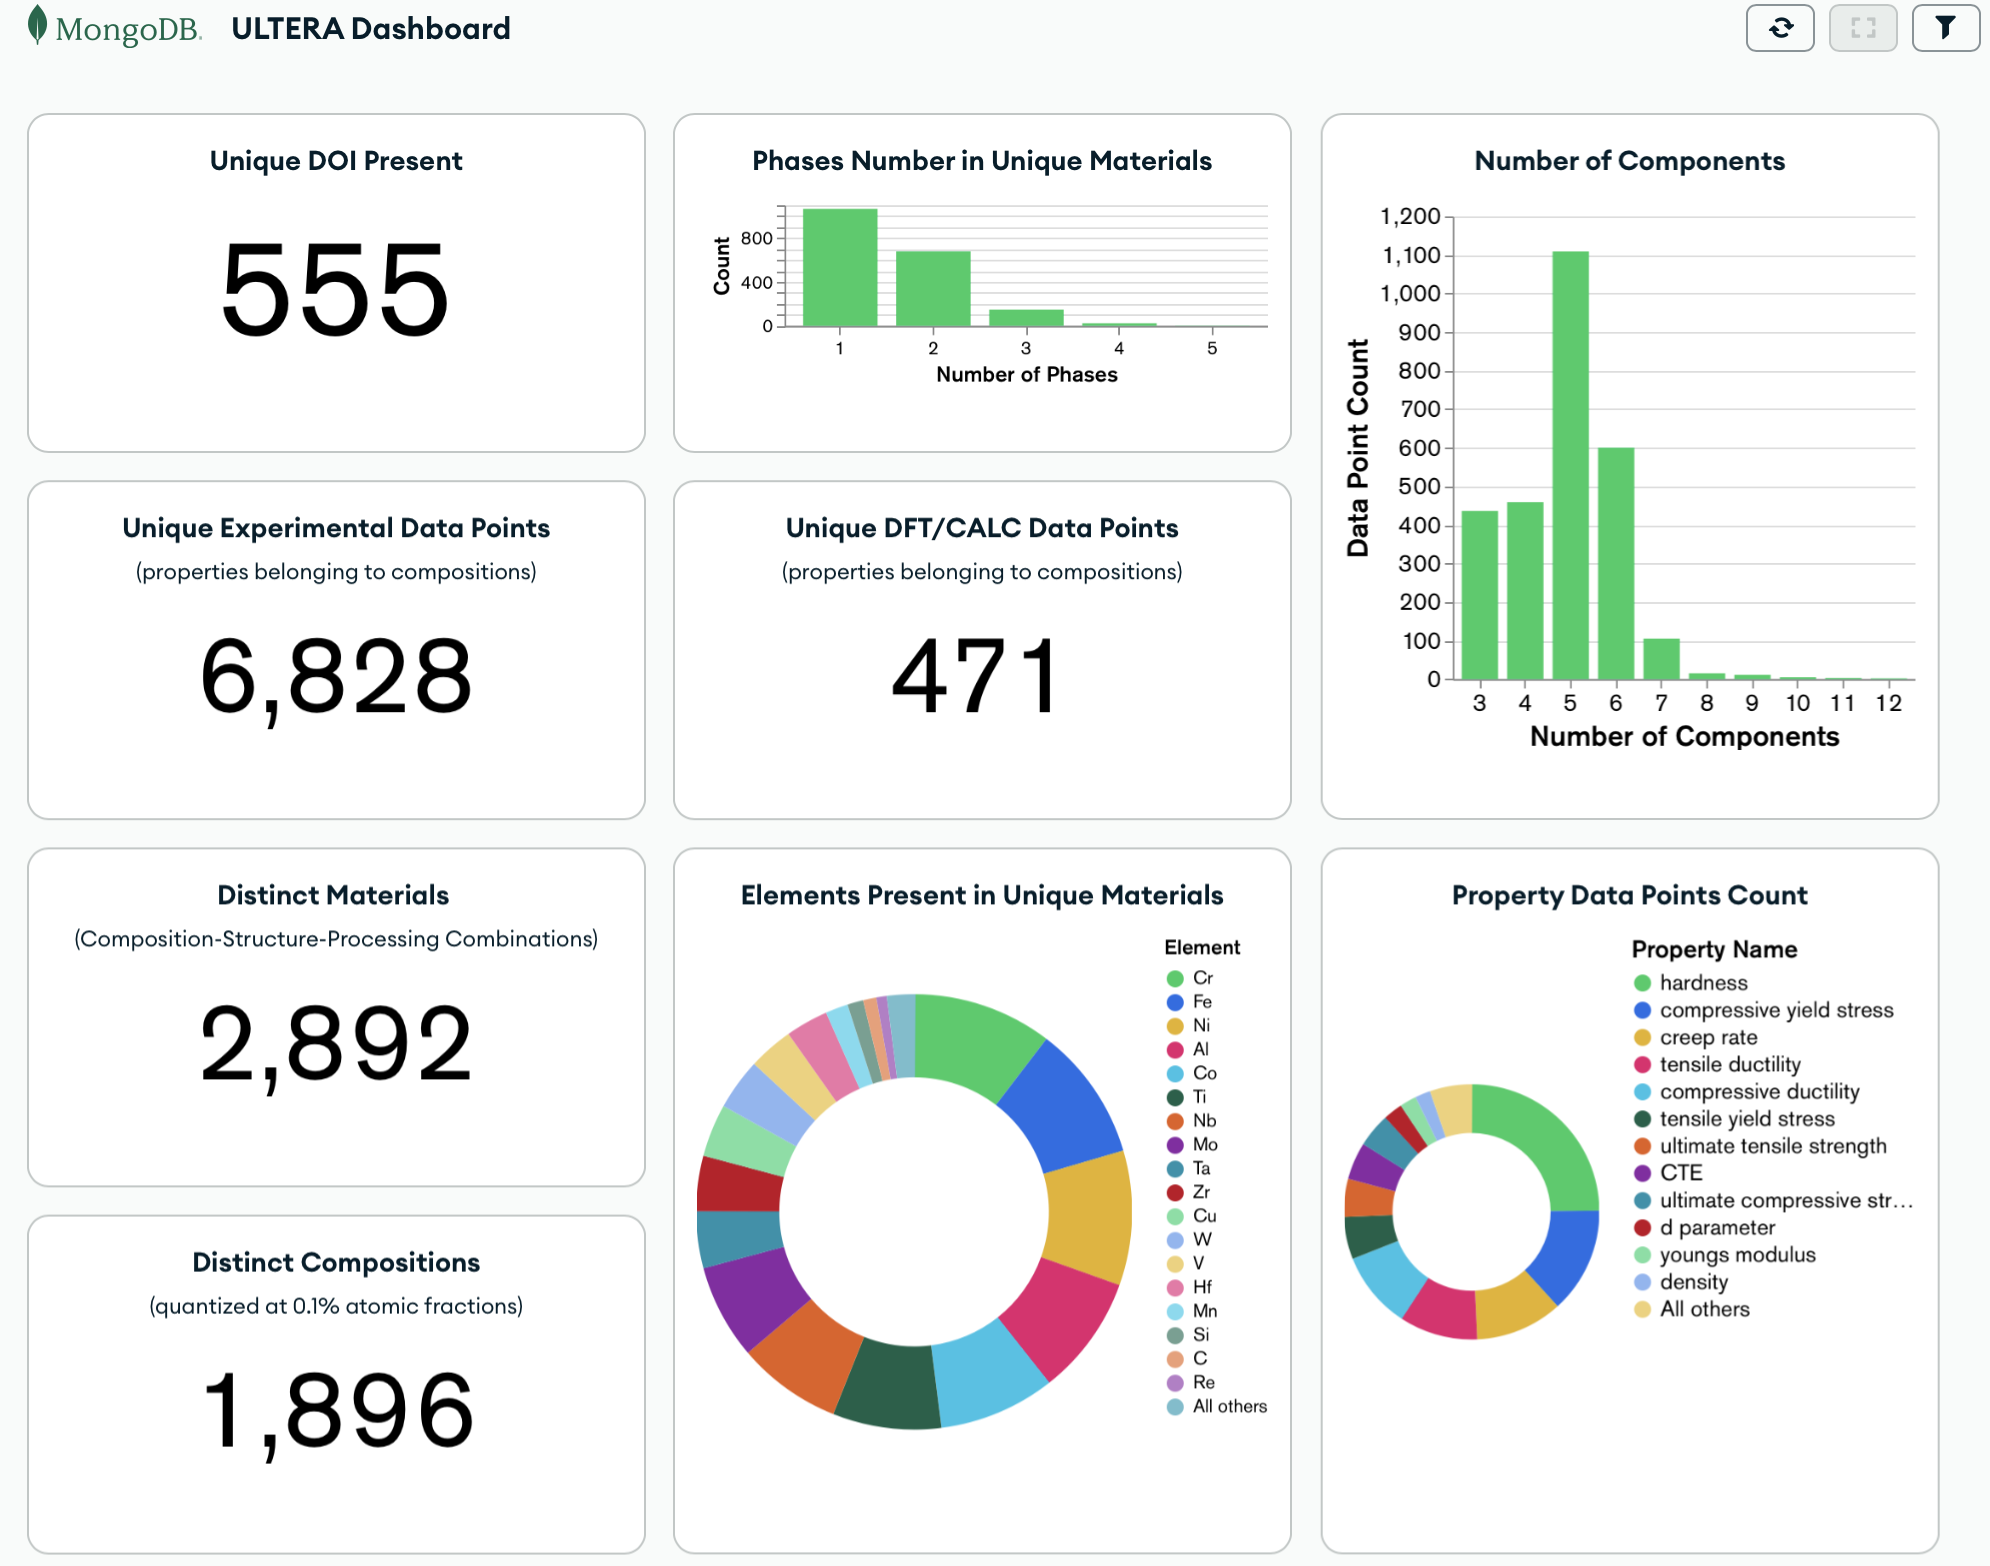
\includegraphics[width=0.95\textwidth]{ultera/ULTERA_Dashboard.png}
    \caption{The main section of \texttt{ULTERA} Database dashboard at \href{https://ultera.org}{ultera.org}; presents statistics as of \statisticstime. All included figures are live and automatically recalculated every 1h. They are interactive allowing users to, e.g., select, highlight, or export the plot data in machine-readable format.}
    \label{ultera:fig:dashboard}
\end{figure}


\begin{figure}[H]
    \centering
    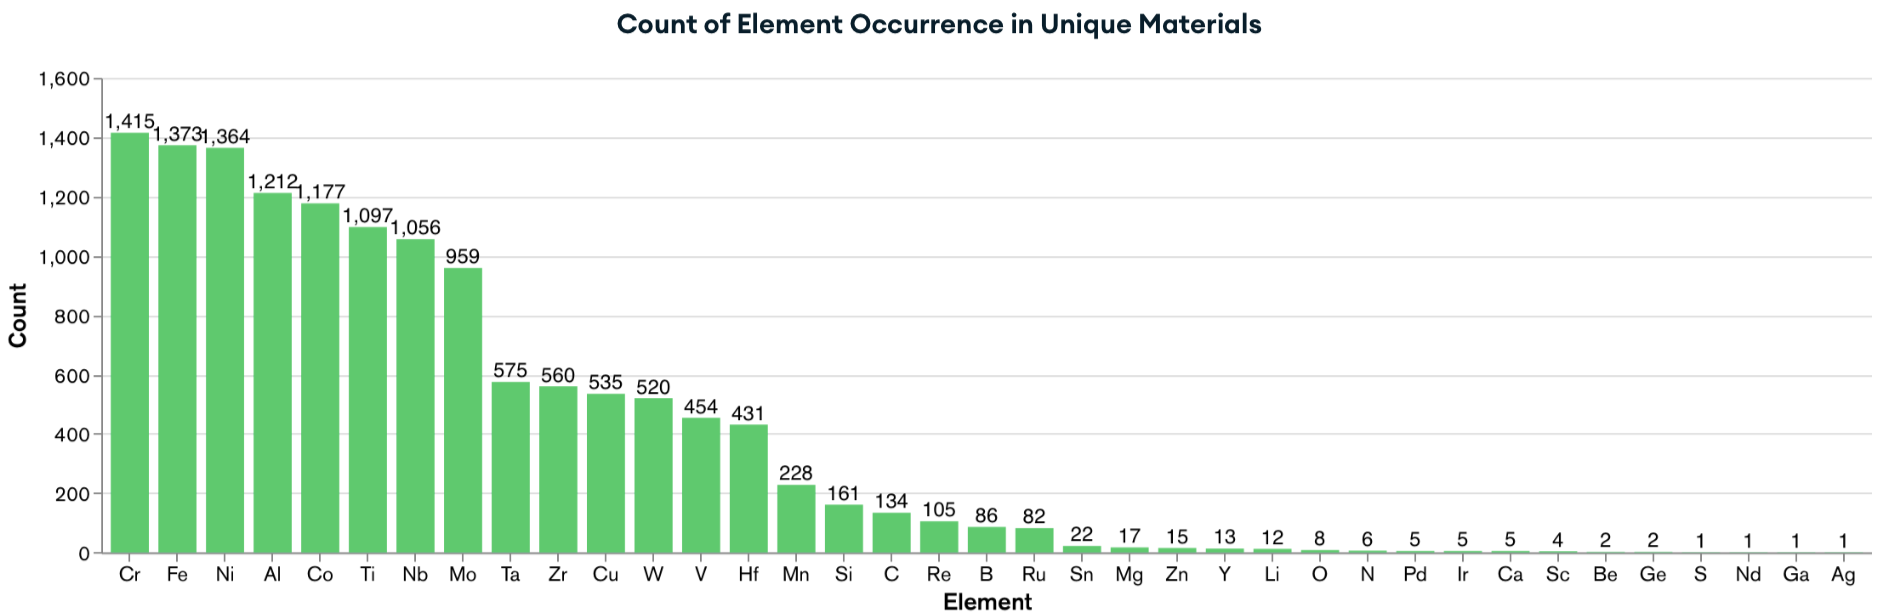
\includegraphics[width=0.95\textwidth]{ultera/ultera_Chemistries.png}
    \caption{Chemical elements in the unique materials collection of the ULTERA Database as of \statisticstime. Please note that the same formula-processing-structure triplet can often be reported by many groups and is counted here as 1 point.}
    \label{ultera:fig:chemistries}
\end{figure}


\begin{figure}[H]
    \centering
    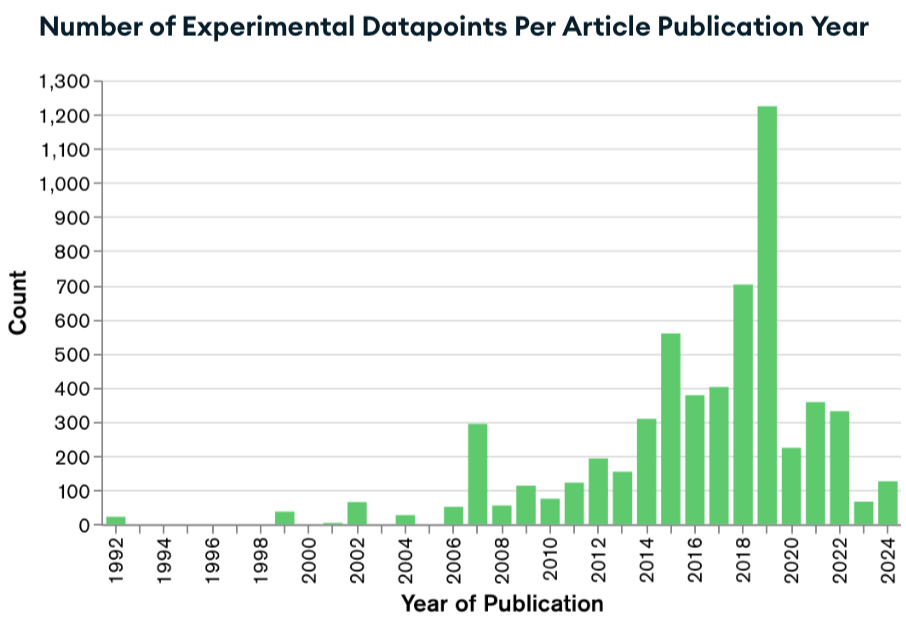
\includegraphics[width=0.5\textwidth]{ultera/ultera_PublicationYear.png}
    \caption{Number of experimental datapoints collected in ULTERA as of \statisticstime vs the year they were published, showing rapid growth. The lower numbers in the last 5 years reported can be attributed to significant portion of the data coming from compilations delayed by 1-3 years and height of COVID pandemic in 2020 delaying experiments.}
    \label{ultera:fig:publicationyears}
\end{figure}


\begin{figure}[H]
    \centering
    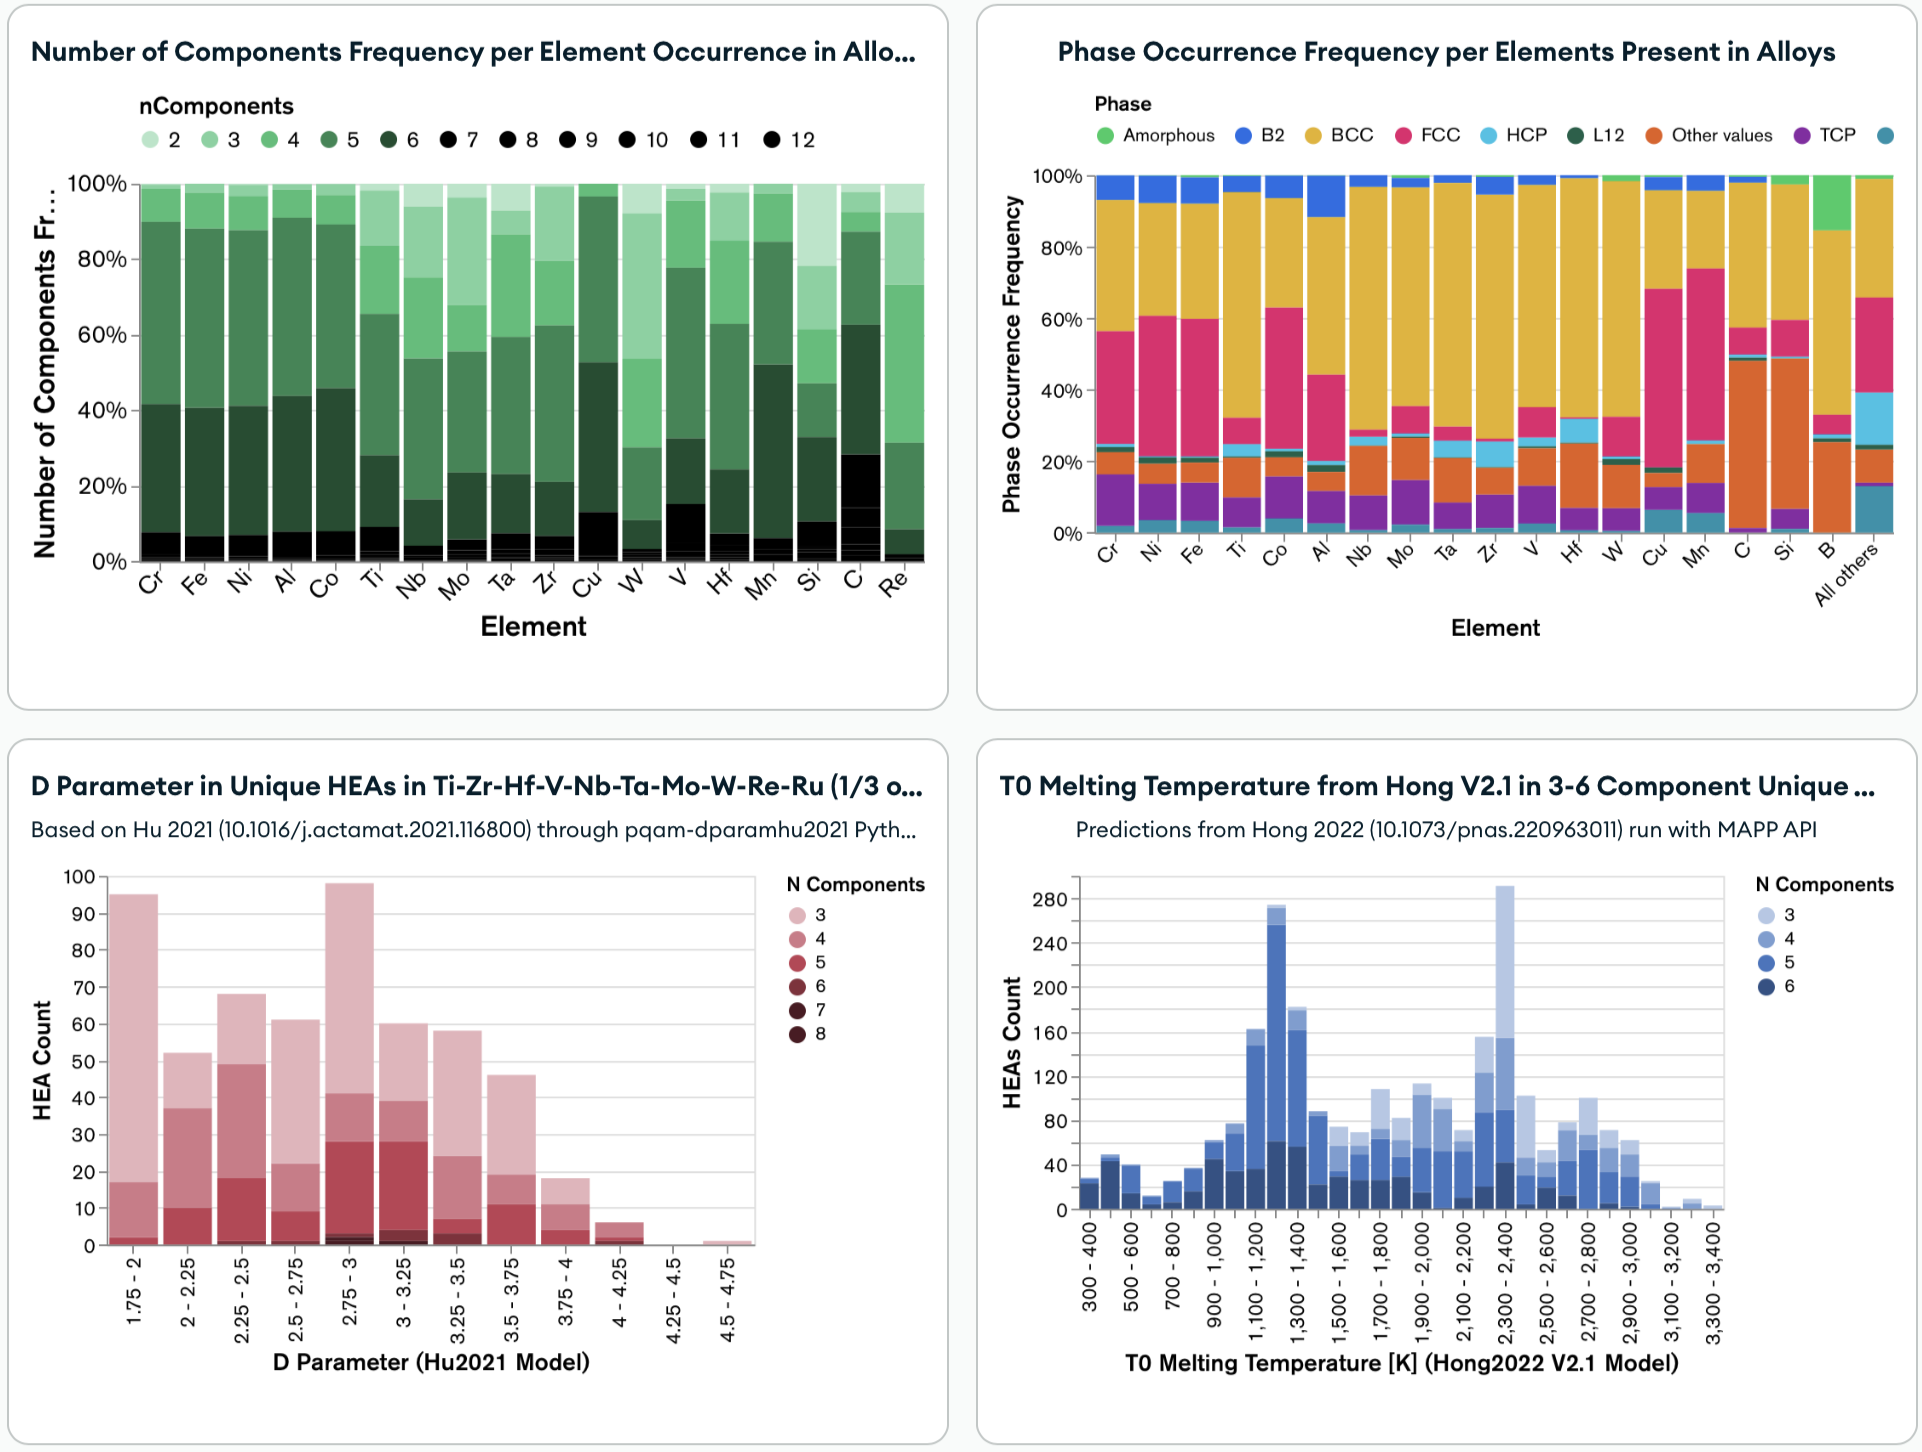
\includegraphics[width=0.95\textwidth]{ultera/ULTERA_Insights.png}
    \caption{A large compiled dataset allows insights into prior expert knowledge driving the discovery and possible biases models generating new alloys will be subject to. The automated data infrastructure, described in Section \ref{ultera:sec:infrastructure}, enables efficient deployment of many tools, such as community models described in Subsection \ref{ultera:ssec:communitymodels}.}
    \label{ultera:fig:insights}
\end{figure}



\section{Alloy Discovery Infrastructure} \label{ultera:sec:infrastructure}

\todo

\begin{figure}[H]
    \centering
    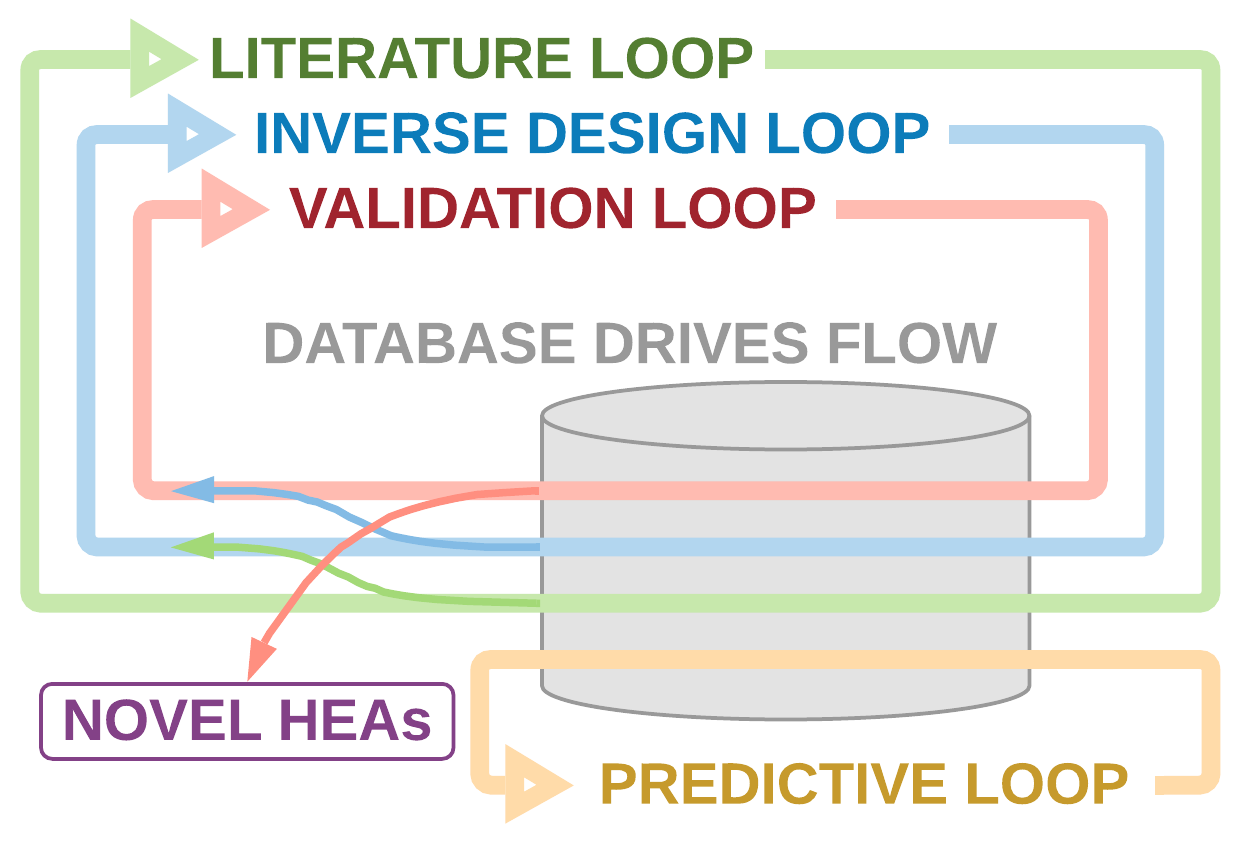
\includegraphics[width=0.5\textwidth]{ultera/PersepctivePaper_DataFlow_V2.png}
    \caption{Four \emph{data loops} associated with different parts of the alloy discovery efforts and the database driving information flow between them to arrive at novel high entropy alloys.}
    \label{ultera:fig:dataloops}
\end{figure}

\begin{figure}[H]
    \centering
    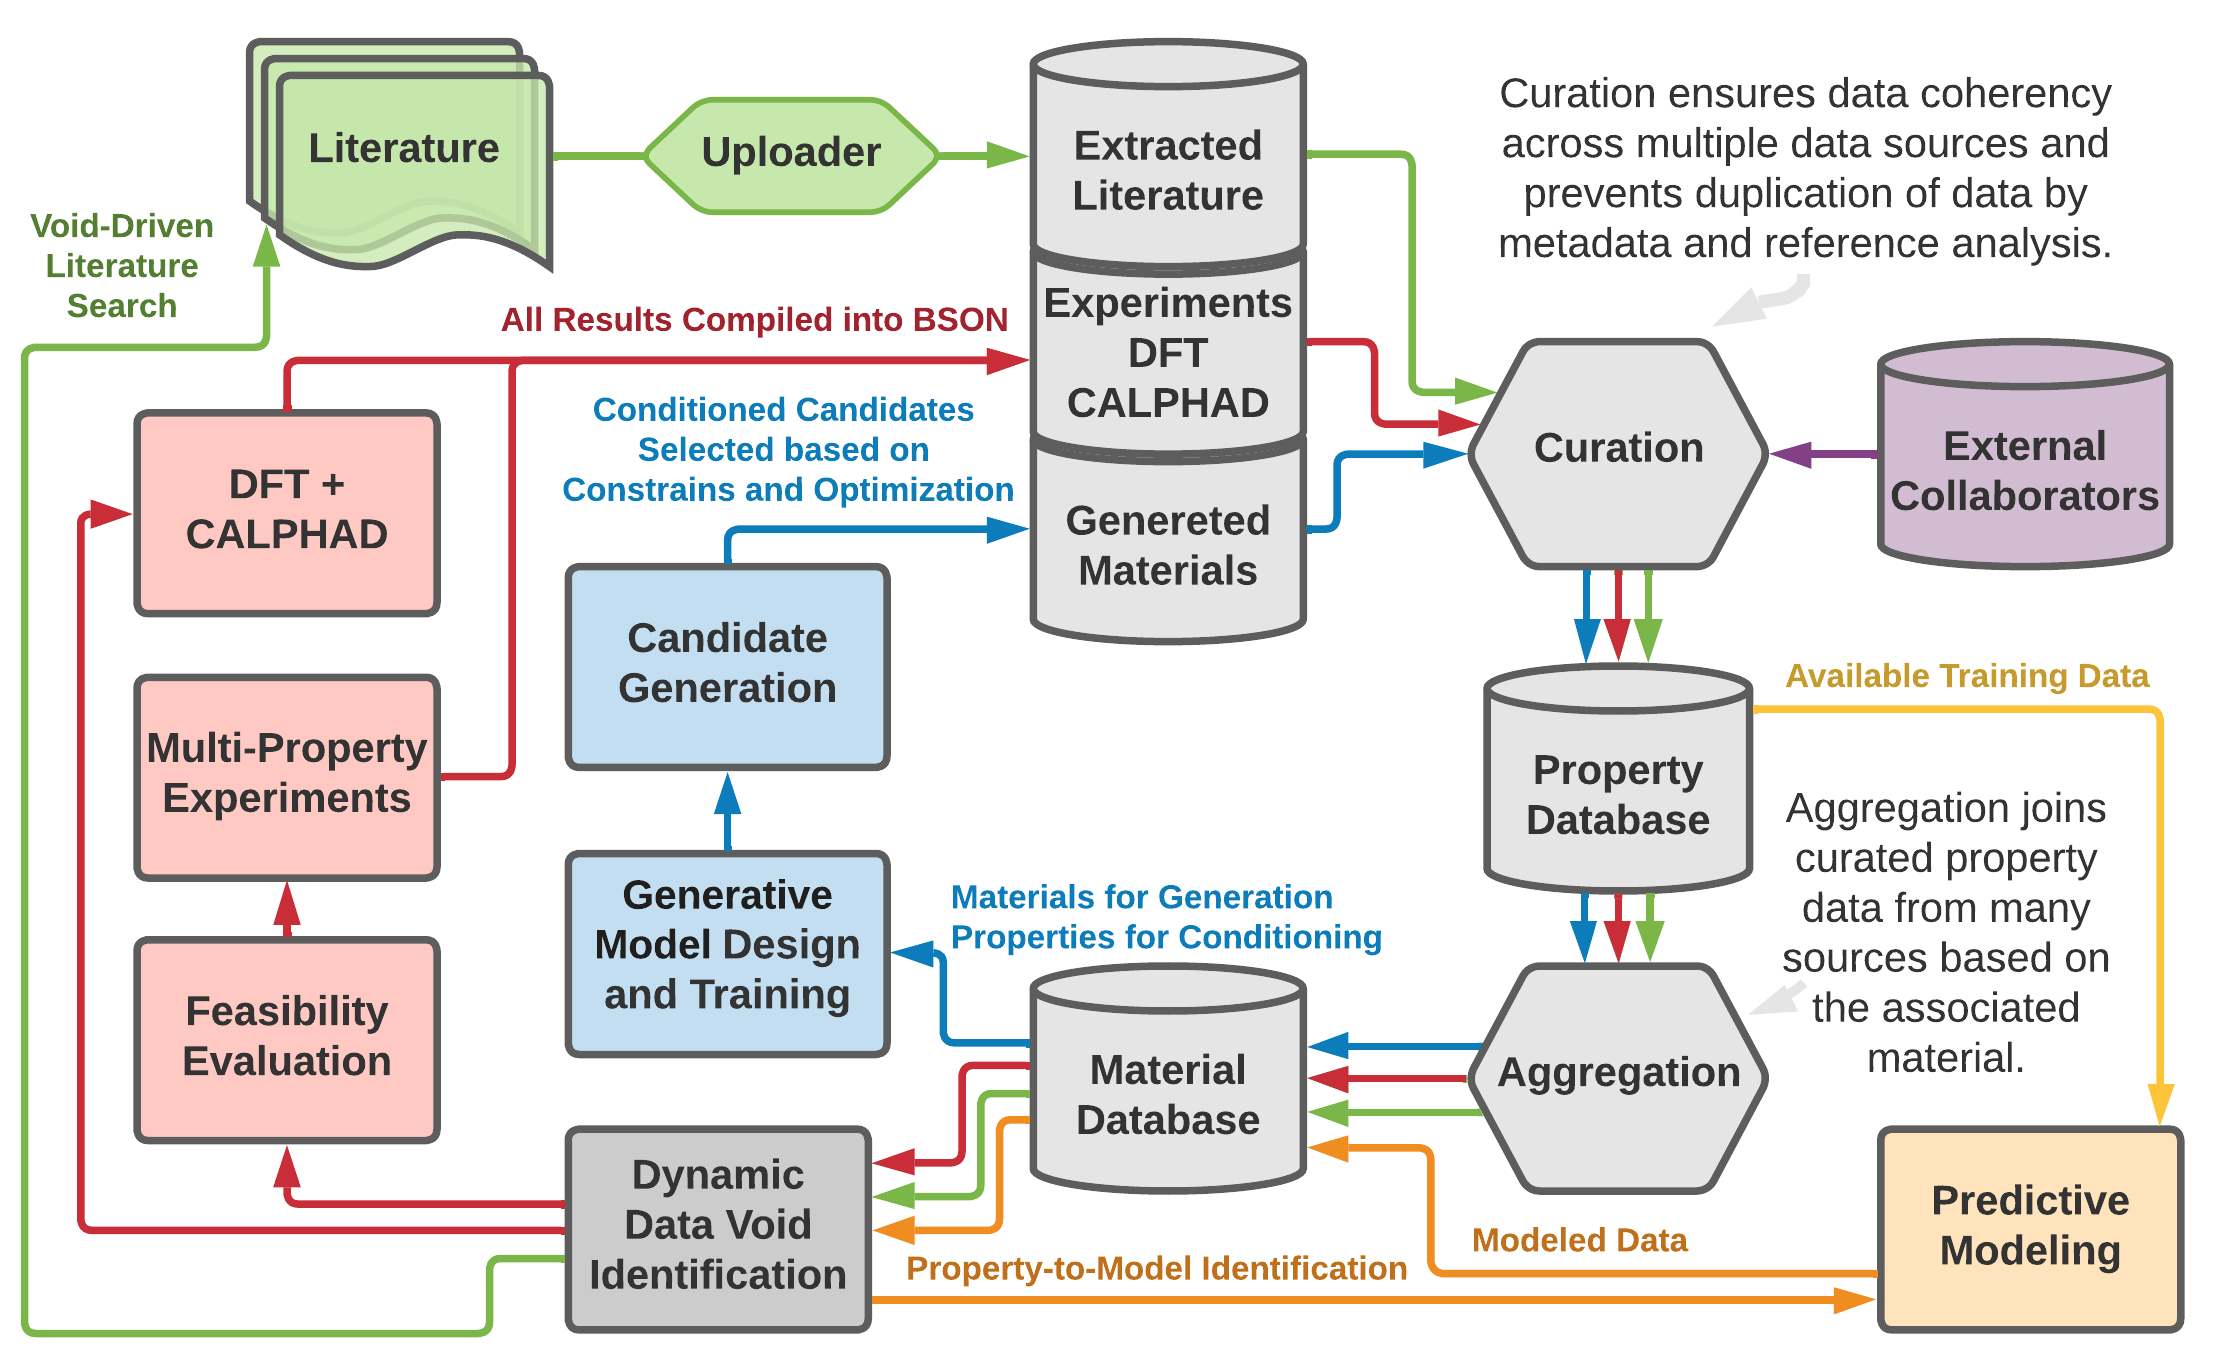
\includegraphics[width=0.9\textwidth]{ultera/PersepctivePaper_Ecosystem_V6.png}
    \caption{Big picture schematic of the ULTERA Data Infrastructure composed of the literature loop (green) collecting available external knowledge from many sources, the predictive loop (orange) filling in the gaps in current state of knowledge with modeling data, the generative loop (blue) proposing new candidate alloys to evaluate, validation loop (red) performing calculations and experiments to validate candidates. In the process databases are created, containing \texttt{CURATED} subset of materials property data, then \texttt{AGGREGATED} around unique materials for multi-property learning. The underlying infrastructure includes many more data collections hidden from users to enable efficient pipelines.}
    \label{ultera:fig:dataschematic}
\end{figure}




\section{Data Pipeline} \label{ultera:sec:pipeline}

\todo

\begin{figure}[H]
    \centering
    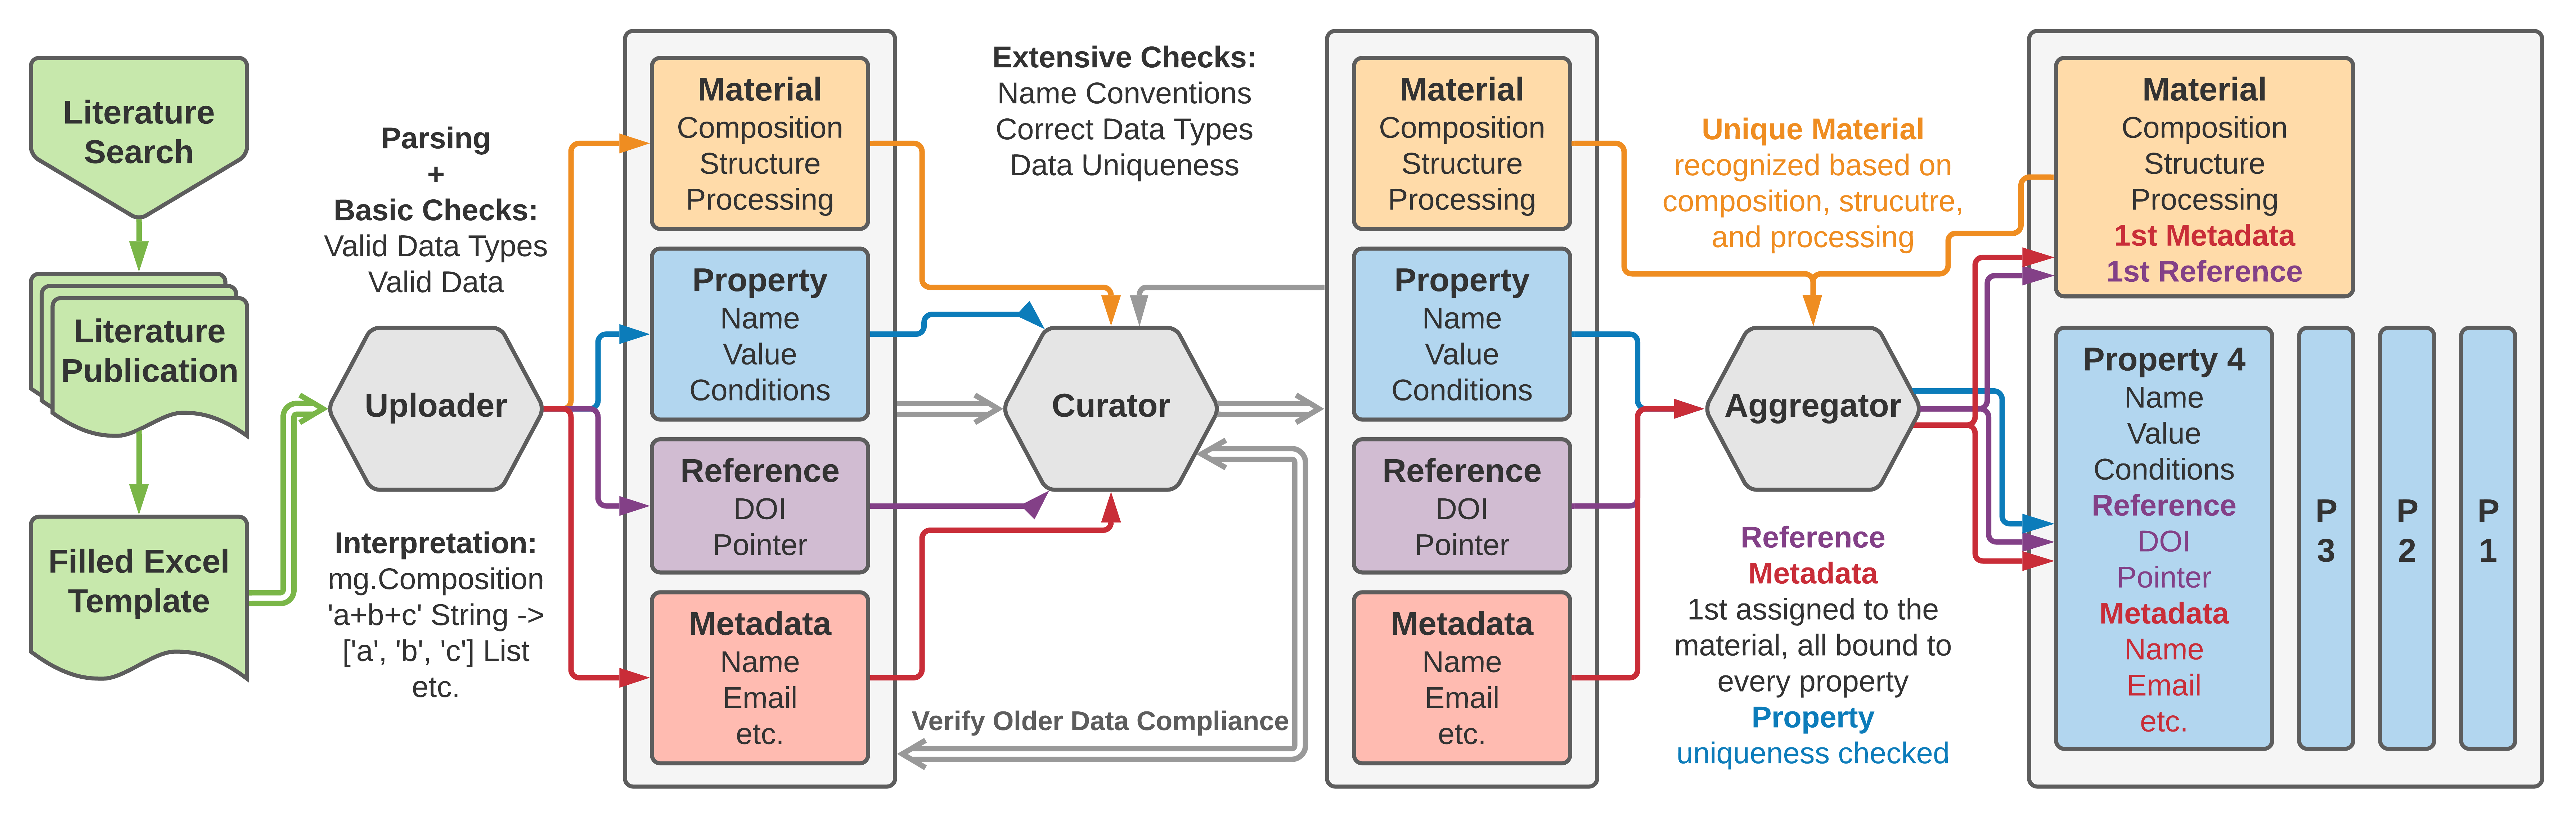
\includegraphics[width=0.95\textwidth]{ultera/ULTERA Data Detail.png}
    \caption{Schematic of the forward pipeline applied to data ingested into the system. For conciseness, intermediate steps of curation process and associated intermediate datasets are not depicted. Critically, a number of data points can converge at each step, so backward trace would be highly branched.}
    \label{ultera:fig:datapipeline}
\end{figure}


\begin{figure}[H]
    \centering
    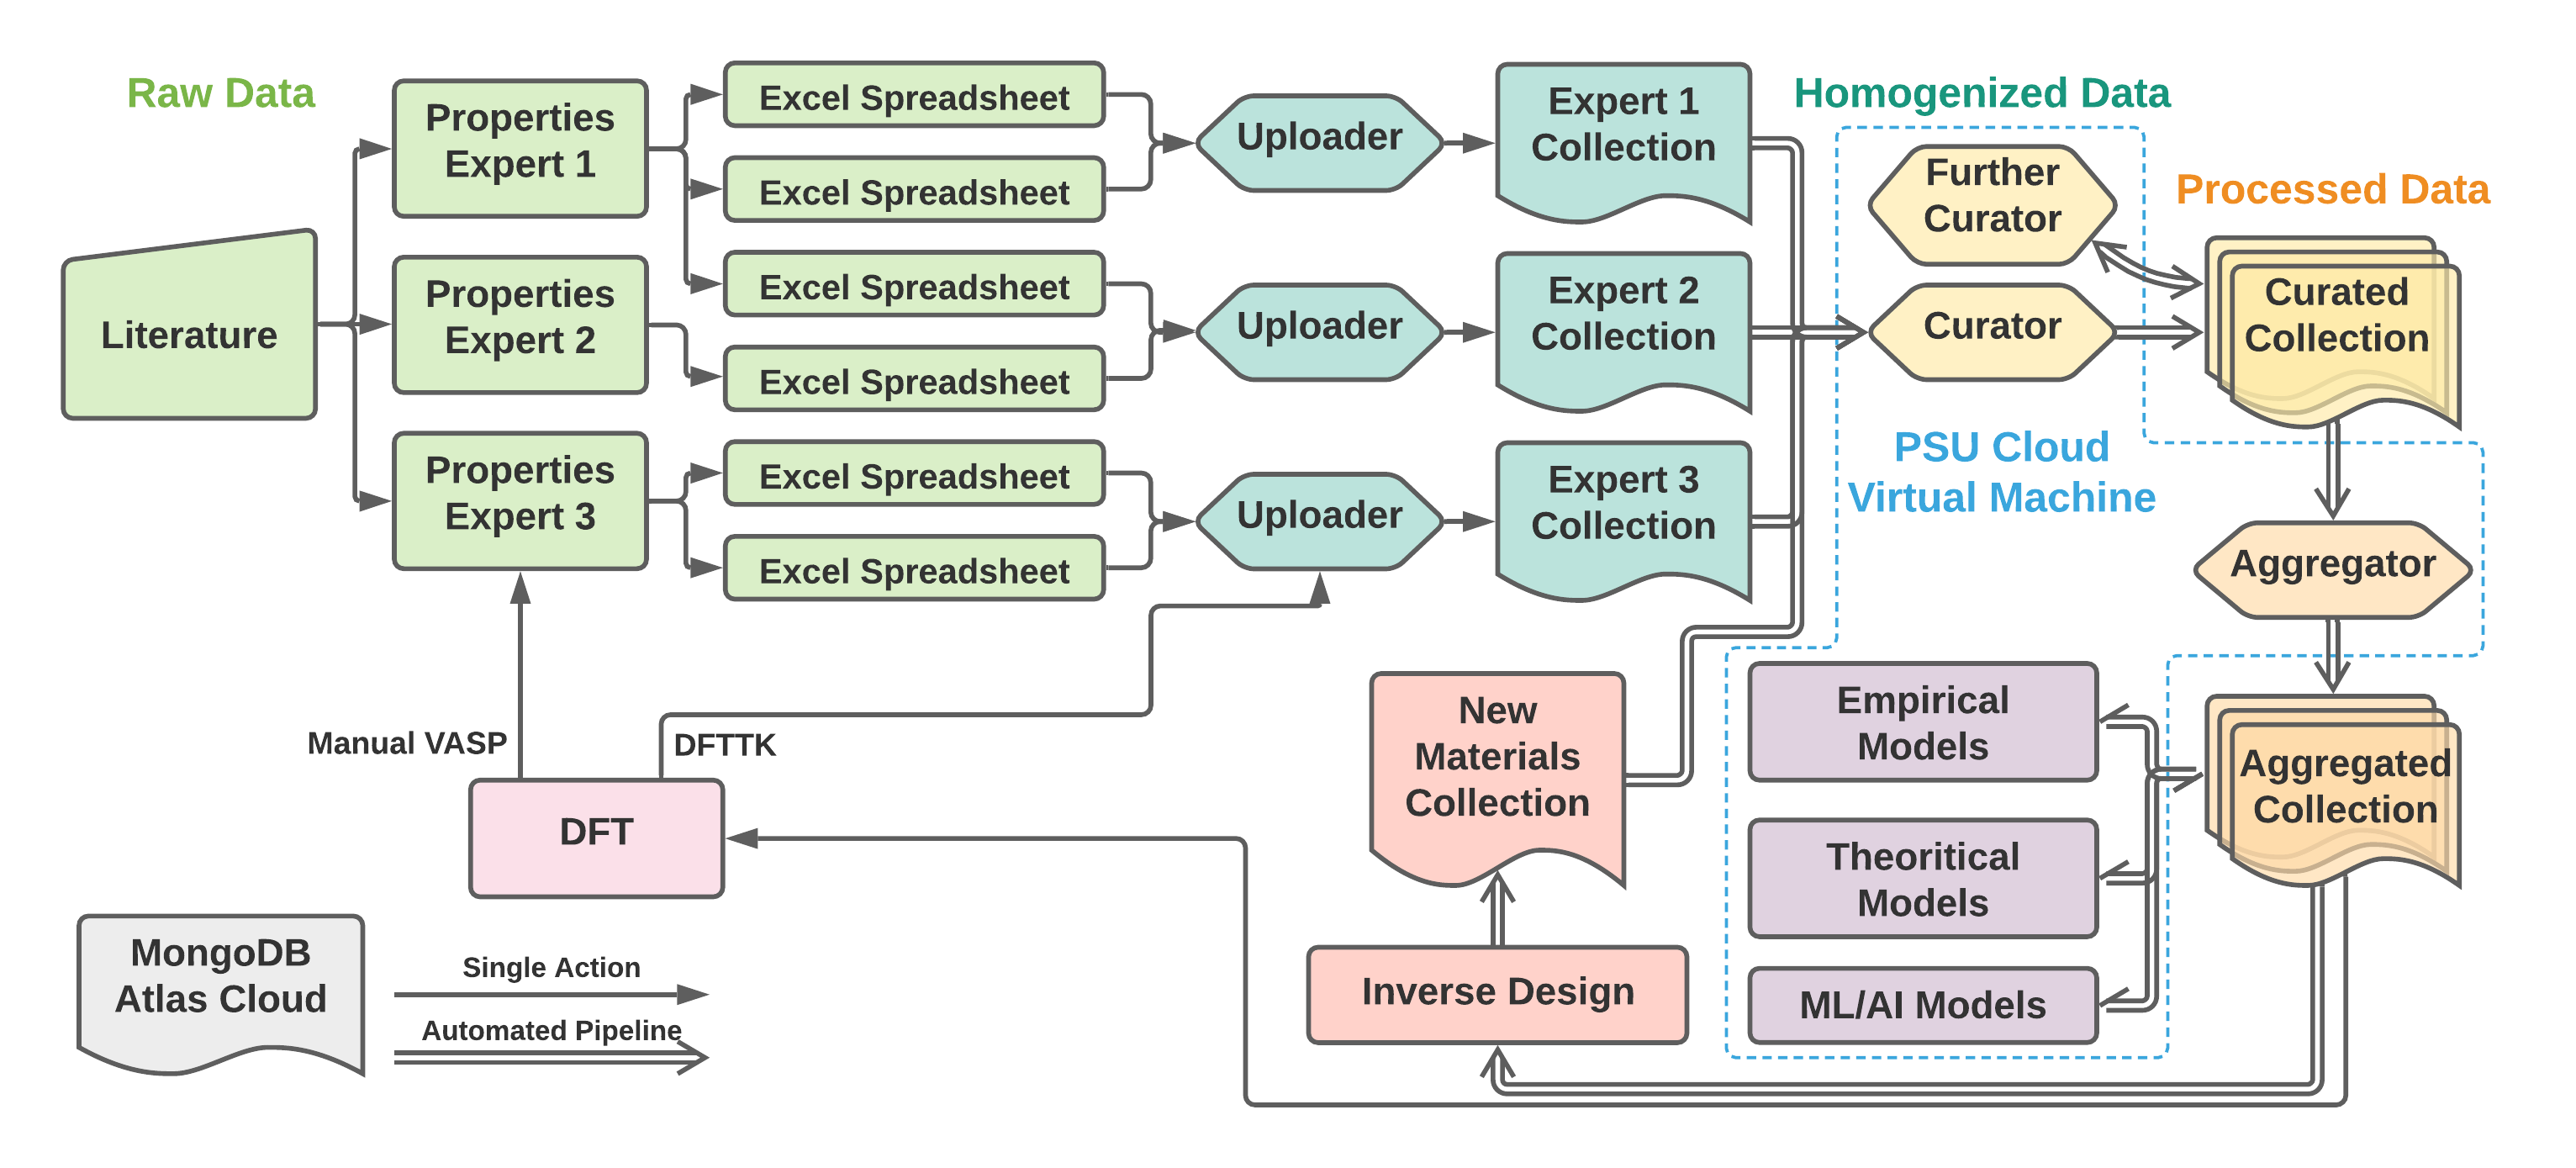
\includegraphics[width=0.95\textwidth]{ultera/ULTERA_Data_Cycle_v2.png}
    \caption{Schematic of the computational (non-experimental) data flow from perspective closer to the underlying pipelines, with double lines marking fully automated steps happening on the cloud. For conciseness, intermediate steps, like reorientation of data around unique compositional or structural datasets for efficient model deployment are not depicted.}
    \label{ultera:fig:datacycles}
\end{figure}




\section{Community Contributions} \label{ultera:sec:contributions}

\todo



\begin{figure}[H]
    \centering
    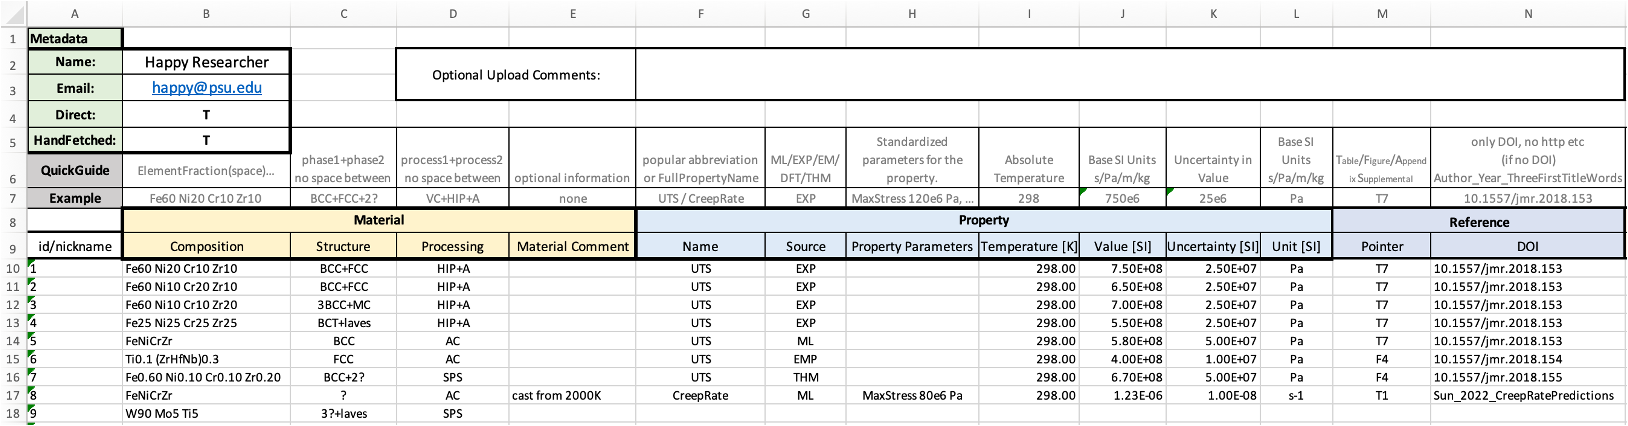
\includegraphics[width=0.95\textwidth]{ultera/ULTERA_Contribute.png}
    \caption{Header and example data rows of a formatted Excel spreadsheet template used to streamline and increase accessibility to the contribution system for non-technical members of the community. An automated system processes them on the cloud into git-tracked plain-text CSV records then passed to uploading system.}
    \label{ultera:fig:contributiontemplate}
\end{figure}




\section{Automatic Modeling} \label{ultera:sec:automodel}

\subsection{Multi-Structure Linear Combinations} \label{ultera:ssec:autolc}

\cite{Chong2021CorrelationAlloys}

\begin{figure}[H]
    \centering
    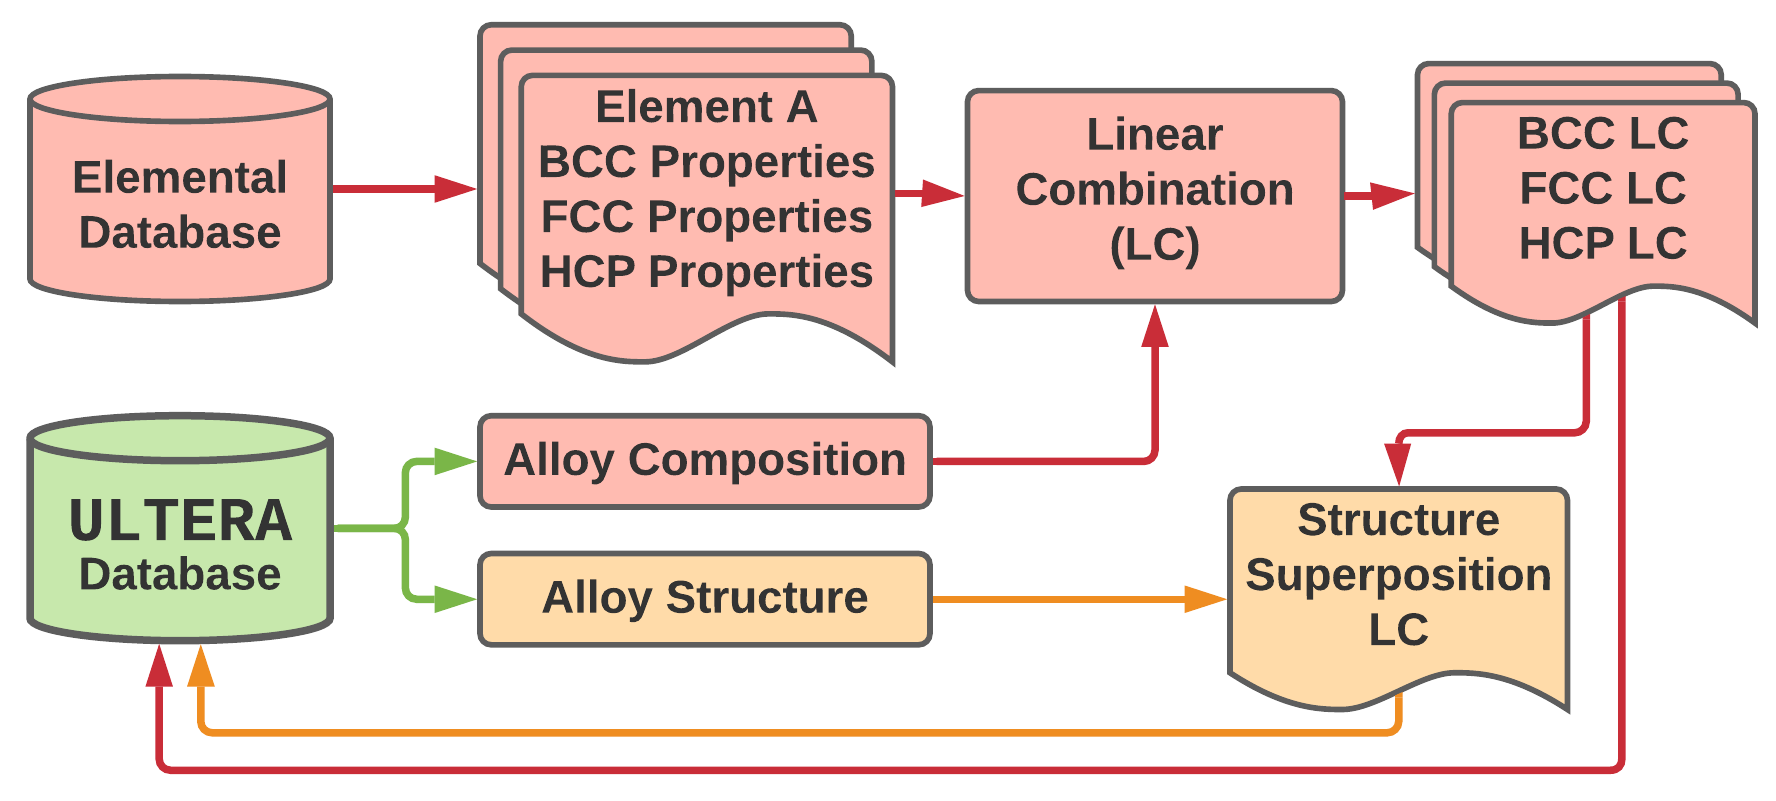
\includegraphics[width=0.6\textwidth]{ultera/ULTERA_ElementalDatabase_LC_V1.png}
    \caption{Simplified schematic of automatic linear combination modeling of properties. For every chemical composition, a linear combination of elemental properties is calculated for BCC, FCC, and HCP structures, based on best-matched elemental polymorph data coming from experiments and DFT-based pure element calculations. If applicable structure set (e.g., FCC+FCC+HCP) has been reported for a given input datapoint, an average of the respective linear combinations is reported as structure-informed LC.}
    \label{ultera:fig:autolc}
\end{figure}




\subsection{Community Model Deployment} \label{ultera:ssec:communitymodels}

\todo




\subsection{Automated CALPHAD Modeling} \label{ultera:ssec:autocalphad}

\todo






\subsection{MPDD Atomic Configuration Data Fetching} \label{ultera:ssec:mpdd}

\todo

\begin{figure}[H]
    \centering
    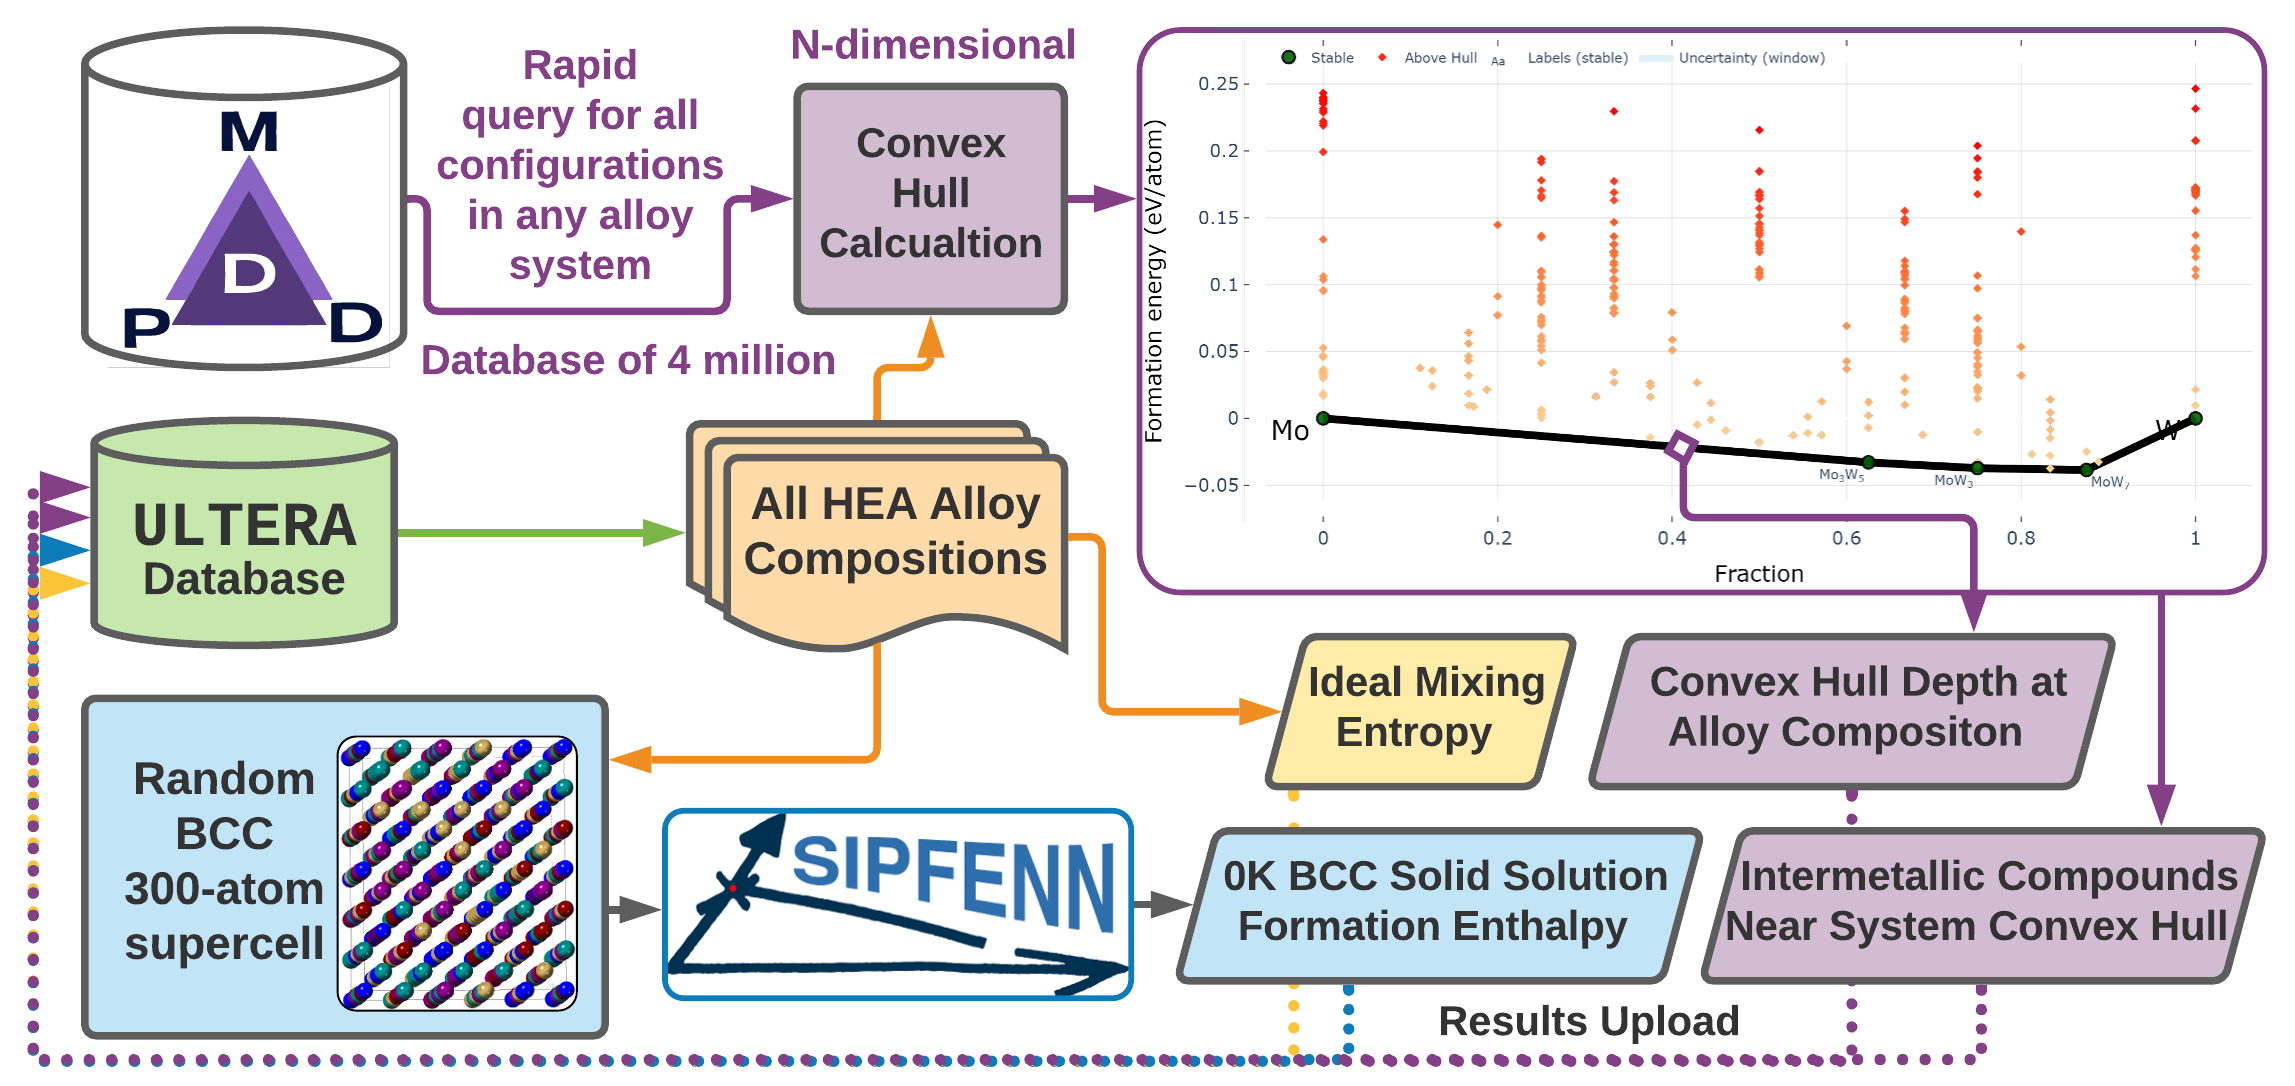
\includegraphics[width=0.6\textwidth]{ultera/ULTERA_BasicThermodynamics_V1.png}
    \caption{Conceptual schematic of how MPDD is directly utilized within ULTERA, going beyond interaction through CALPHAD models, to include basic thermodynamic information. For each composition, a convex hull of compounds present in corresponding chemical system is calculated based on MPDD data and can be used (a) to immediately identify candidates for experimentally observed compounds based on 0K low-energy configurations or (b) convex hull depth can be used as an input to ML model indicating strength of interatomic interactions.}
    \label{ultera:fig:mpdd}
\end{figure}








\printbibliography[heading=subbibintoc]